% !TeX spellcheck = de_CH
\chapter{Bellsche Ungleichung\label{chapter:bell}}
\lhead{Bellsche Ungleichung}
\begin{refsection}
\chapterauthor{Hannes Badertscher}

In diesem Kapitel betrachten wir ein Theorem von Albert Einstein genauer.
Wie Randall Munroe von xkcd im
Comic~\ref{fig:bell:xkcd_einstein} illustriert konnten die Theorien von
Einstein bisher kaum widerlegt werden.
Als einziges Beispiel Einstein zu widerlegen wird eine m\"oglicherweise falsche
Entscheidung Einsteins, als er bei seiner Arbeit im Patentamt ein umstrittenes
Patent zur Annahme empfahl, aufgef\"uhrt.
Obwohl scheinbar unm\"oglich, befassen wir uns in diesem Kapitel mit der Arbeit
von Albert Einstein und versuchen diese kritisch zu beleuchten.

\begin{figure}[b]
    \centering
    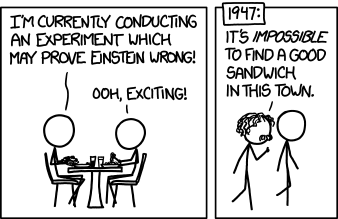
\includegraphics[width=0.5\linewidth]{bell/images/xkcd_einstein.png}
    \caption{XKCD Comic, welches darauf anspielt, dass kaum Fehler 
    in den Arbeiten von Albert Einstein finden lassen \cite{Bell:XkcdComic}}
    \label{fig:bell:xkcd_einstein}
\end{figure}


Im Mai 1935 ver\"offentlichten Albert Einstein, Boris Podolsky und
Nathan Rosen ein Gedankenexperiment mit welchem sie erkl\"arten, wieso
die Quantenmechanik nicht vollst\"andig sein kann. Als Alternative
sollten zus\"atzliche, verborgene, Variablen eingef\"ugt werden, welche
das zugrunde liegende Verhalten logisch erkl\"aren k\"onnen.
Die Theorie der verborgenen lokalen Variablen nach Einstein war lange
die verbreitete Ansicht -- die Frage war nur wann solche Variablen
entdeckt werden. In vielen Bereichen der Quantenmechanik wurden tats\"achlich
kleinere Teilchen, Quantenzahlen und Variablen entdeckt, welche das
Verst\"andnis der heutigen Quantenphysik pr\"agten.

Wir betrachten das Gedankenexperiment von Einstein, indem wir zuerst die
grundlegenden Annahmen der Lokalit\"at und des Realismus betrachten. Danach
gehen wir auf das von Einstein, Rosen und Podolski ver\"offentlichte Paradoxon
ein und kommen auf die darauf basierende Bell'sche Ungleichung, welche
1961 von John Bell ver\"offentlicht wurde.

\section{Lokalit\"at und Realismus\label{section:bell:lokalitaet}}
Zuerst stellt sich die Frage der Anforderungen an die Theorie der
Quantenmechanik. Eine zentrale Eigenschaft ist hierbei die Lokalit\"at.
Lokalit\"at bedeutet hierbei, dass jegliche Vorg\"ange nur einen Einfluss
auf ihre direkte Umgebung haben k\"onnen.

Die klassische Newtonsche Mechanik ist eine \emph{nicht}-lokale 
Theorie. Eine Masse hat in der Gravitation sofort, ohne zeitliche 
Verz"ogerung einen Einfluss auf andere Massen, unabh\"angig von der
r\"aumlichen Distanz zwischen den beiden Massen. 
In der speziellen Relativit\"atstheorie 
\textsuperscript{[Citation needed]}
wurden die Begriffe von Raum und Zeit so definiert, dass sich alle
Materie und Energie sich h\"ochstens mit Lichtgeschwindigkeit fortbewegen
kann. 
Die allgemeine Relativit\"atstheorie ist eine alternative Formulierung
der Newtonschen Gravitationstheorie, welche die in der speziellen
Relativit\"atstheorie geforderte Lokalit\"at erf\"ullt.
Von der Quantenmechanik kann ebenfalls erwartet werden, dass sich
jegliche Ereignisse h\"ochstens mit Lichtgeschwindigkeit ausbreiten
k\"onnen.

Eine Theorie wird als \emph{realistisch} bezeichnet, wenn die Theorie
nicht direkt von der Messung abh\"angt. Eine Messung hat also einen
vordefinierten Wert, auch wenn dieser nicht bekannt ist.
Die bekannte Frage \enquote{Is the moon there if nobody looks?} zeigt auf,
dass der Realismus rein intuitiv immer erf\"ullt sein m\"usste. Schliesslich
zweifelt niemand daran, dass der Mond auch existiert wenn gerade niemand
zum Mond hinaufschaut.

\section{Das Einstein-Podolsky-Rosen Paradoxon}
Das Einstein-Podolsky-Rosen Paradoxon (EPR Paradoxon) ist ein 
Gedankenexperiment, welches 1935 im Paper \cite{Bell:Einstein1935}
\emph{Can quantum-mechanical description of physical reality be considered complete}
von Albert Einstein, Boris Podolsky und Nathan Rosen publiziert wurde.
Wie der Titel bereits verr\"at, gehen Einstein \emph{et al.} dabei auf
zwei Fragen ein: 
(1) \enquote{Ist die Theorie korrekt?}
und 
(2) \enquote{Ist die Beschreibung durch die Theorie vollst\"andig?}
Nur wenn beide diese Fragen mit \emph{ja} beantwortet werden k\"onnen, kann
eine Theorie die Realit\"at zufriedenstellend beschreiben.
Die erste Frage kann einfach gepr\"uft werden, indem die Resultate von
Experimenten mit den Vorhersagen der Theorie verglichen werden. 
Die Quantenmechanik konnte dabei in zahlreichen Experimenten die Wirklichkeit
vorhersagen. 
Einstein, Rosen und Podolski befassten sich deshalb mehr mit der zweiten
Frage. 
Die Vollst\"andigkeit einer Theorie wird dabei wie folgt definiert:

\begin{definition}\label{def:Bell:Vollstaendigkeit}
    Jedes Element der physikalischen Realit\"at muss durch die Theorie
    genau beschrieben werden k\"onnen.
\end{definition}

Während Einstein \emph{et al.} in ihrem Paper das Gedankenexperiment sehr
allgemein halten, betrachten wir hier ein anschaulicheres Beispiel, welches
1957 von David Bohm und Yakir Aharonov \cite{Bell:Bohm1957} pr\"sentiert wurde.

\subsection{Das Gedankenexperiment}
Wir betrachten zwei quantenmechanische Systeme, $I$ und $II$,
welche von $t=0$ bis zu einem Zeitpunkt $t=T$ miteinander 
interagieren k\"onnen. Darauf ist keine Interaktion mehr m\"oglich.
Visualisiert wird das Gedankenexperiment durch eine Quelle, welche
Elektron-Positron Paare emittiert. 
Dabei wird das Elektron ($I$) zu einem Detektoren $A$ und das 
Positron ($II$) zu einem Detektoren $B$ gesandt.
Diese sind physikalisch getrennt, sodass kein Informationsaustausch
zwischen den Detektoren m\"oglich ist.
Der Messaufbau ist in \figurename~\ref{fig:bell:EPR_Messaufbau} abgebildet.

\begin{figure}
    \centering
    \includegraphics{bell/images/experiment_setup.pdf}
    \caption{Messaufbau im Gedankenexperiment von EPR}
    \label{fig:bell:EPR_Messaufbau}
\end{figure}

Diese zwei Partikel werden so generiert, dass sie einen komplement\"aren
Spin-Zustand besitzen. 
Wenn also bei Detektor $A$ der Spin des Elektrons entlang der $z$-Achse
gemessen wird und das Messresultat $+z$ ist, so ist sofort klar, dass
das das Positron bei Detektor $B$ den Spin $-z$ besitzen muss. 
Ebenso wird, falls bei Detektor $A$ der Spin entlang der $x$-Achse als $+x$
gemessen wird, das Positron bei Detektor $B$ den Spin $-x$ besitzen.

Wie im Kapitel der Heisenbergschen Unsch\"arferelation
\textsuperscript{[Citation needed]}
erkl\"art wird, sind die Messungen des Spins in verschiedenen Dimensionen 
komplement\"are Operatoren.
Damit ist es unm\"oglich, gleichzeitig beide Eigenschaften eines Teilchens
beliebig genau zu kennen.
Wird nun jedoch bei Detektor $A$ der Spin des Elektrons in $z$-Richtung 
als $+z$ gemessen, so ist bekannt dass das Positron den Spin $-z$ besitzt.
Da jedoch noch keine Messung am Positron ausgef\"uhrt wurde, kann bei
Detektor $B$ der Spin in $x$-Richtung gemessen werden.
Es ist also m\"oglich f\"ur das Positron gleichzeitig die exakten Werte 
des Spins in $x$-, wie in $z$-Richtung zu kennen. 
Mit der uns bekannten Beschreibung der Quantenmechanik mit Wellenfunktionen
kann dieser Effekt \emph{nicht} beschrieben werden, womit wir zu der
logischen Schlussfolgerung Einsteins kommen:

\begin{satz}
    Die quantenmechanische Beschreibung der physikalischen Realit\"at mittels
    Wellenfunktionen ist keine vollst\"andige Theorie.
\end{satz}

\subsection{Mathematische Herleitung}
Anhand des Spins kann das EPR Paradoxon einfach mathematisch formuliert werden.
Dabei wird die Notation aus Kapitel~\ref{chapter:spin}~\nameref{chapter:spin}
verwendet.

Wie in den Gleichungen~\ref{spin:paulimatrizen}--\ref{spin:vektoroperator}
hergeleitet wird der Spin-Operator durch die hermiteschen Pauli-Matrizen
beschrieben.

\begin{align*}
    S_1 &= \frac{\hbar}{2} \begin{pmatrix}
    0 & 1 \\ 1 & 0
    \end{pmatrix}
    &
    S_2 &= \frac{\hbar}{2} \begin{pmatrix}
    0 & -i \\ i & 0
    \end{pmatrix}
    &
    S_3 &= \frac{\hbar}{2} \begin{pmatrix}
    1 & 0 \\ 0 & -1
    \end{pmatrix}
\end{align*}

Die zugeh\"origen Eigenvektoren wurden in einer \"Ubung hergeleitet und
betragen:
\begin{align*}
    |{+}x\rangle &= \frac{1}{\sqrt{2}}\begin{pmatrix} 1\\1 \end{pmatrix} &
    |{-}x\rangle &= \frac{1}{\sqrt{2}}\begin{pmatrix} 1\\-1 \end{pmatrix} &
    |{+}y\rangle &= \frac{1}{\sqrt{2}}\begin{pmatrix} 1\\i \end{pmatrix} &
    |{-}y\rangle &= \frac{1}{\sqrt{2}}\begin{pmatrix} i\\1 \end{pmatrix} &
    |{+}z\rangle &= \begin{pmatrix} 1\\0 \end{pmatrix} &
    |{-}z\rangle &= \begin{pmatrix} 0\\1 \end{pmatrix} &
\end{align*}

Der Spin entlang der $z$-Achse eines Elektron-Positron Paares $|\psi\rangle$
kann durch alle m\"oglichen Kombination der beiden Spins von Elektron und
Positron beschrieben werden. Diese umfassen $+z$ f\"ur das Elektron und $-z$
f\"ur das Positron, sowie $-z$ f\"ur das Elektron und $+z$ f\"ur das Positron:
\begin{equation}
    |\psi\rangle = \frac{1}{\sqrt{2}} \Big( 
        |{+}z\rangle \otimes |{-}z\rangle - |{-}z\rangle \otimes |{+}z\rangle
     \Big)
\end{equation}
Damit gilt
%TODO: vielleicht noch ein paar Klammern spendieren.
\begin{align}
    |\psi\rangle &= \frac{1}{\sqrt{2}} 
    \left( 
        \begin{pmatrix} 1\\0 \end{pmatrix} 
        \otimes 
        \begin{pmatrix} 0\\1 \end{pmatrix}
        -
        \begin{pmatrix} 0\\1 \end{pmatrix}
        \otimes
        \begin{pmatrix} 1\\0 \end{pmatrix}
     \right)
     =
     \frac{1}{\sqrt{2}}\left(
         \begin{pmatrix} 0 \\ 1 \\ 0 \\ 0 \end{pmatrix}
         -
         \begin{pmatrix} 0 \\ 0 \\ 1 \\ 0 \end{pmatrix}
     \right)
     = 
     \frac{1}{\sqrt{2}}\left(
         \frac{1}{2}
         \begin{pmatrix} \phantom{-}1 \\ \phantom{-}1 \\ -1 \\ -1 \end{pmatrix}
         -
         \frac{1}{2}
         \begin{pmatrix} \phantom{-}1 \\ -1 \\ \phantom{-}1 \\ -1 \end{pmatrix}
     \right) \\
     &=
    -\frac{1}{\sqrt{2}} \left( 
        \frac{1}{\sqrt{2}}\begin{pmatrix} 1 \\ 1 \end{pmatrix} 
        \otimes 
        \frac{1}{\sqrt{2}}\begin{pmatrix} \phantom{-}1 \\ -1 \end{pmatrix}
        -
        \frac{1}{\sqrt{2}}\begin{pmatrix} \phantom{-}1 \\ -1 \end{pmatrix}
        \otimes
        \frac{1}{\sqrt{2}}\begin{pmatrix} 1 \\ 1 \end{pmatrix} 
     \right) \\
      &= 
      -\frac{1}{\sqrt{2}} \Big( 
              |{+}x\rangle \otimes |{-}x\rangle - |{-}x\rangle \otimes |{+}x\rangle
           \Big)
\end{align}

%TODO: Aussage: here's the magic! das kann nicht sein!!!!!!

Mit der Messung des $z$-Spins bei Detektor $A$ wird eine Projektion auf
entweder $|{+}z\rangle$ oder $|{-}z\rangle$ gemacht, womit der Zustand
$|\psi\rangle$ auf
\[
    |{+}z\rangle \otimes |{-}z\rangle
\]
respektive
\[
    |{-}z\rangle \otimes |{+}z\rangle
\]
reduziert wird.
Das Ergebnis einer Messung $S_z$ bei Detektor $B$ ist damit sofort, 
ohne \"uberhaupt eine Messung durchf\"uhren zu m\"ussen, bekannt und wird
$-z$ resp. $+z$ ergeben.

%TODO: kommuntatoren einfügen

\subsection{Verborgene lokale Variablen}
Die verbreitete Erkl\"arung zur L\"osung des EPR Paradoxons war die Theorie
der verborgenen, lokalen Variablen. Damit sind generell Theorien gemeint,
welche die Zuf\"alligkeiten der Quantenmechanik durch das Einf\"uhren von
zus\"atzlichen Variablen eliminieren. Da zu diesem Zeitpunkt keine solchen
gemessen werden konnten, wurden diese als \emph{verborgene}
Variablen bezeichnet. Weiter wird verlangt, dass diese Variablen sowohl
die Forderungen an Lokalit\"at wie auch Realismus erf\"ullen.

F\"ur das Beispiel des Elektron-Positron Paares ist eine 
einzelne 3-dimensionale Variable $\lambda$ ausreichend um jegliche
Kombinationen zwischen Spin $+$ und $-$ in allen 3 Dimensionen 
$x$, $y$ und $z$ abdecken zu k\"onnen.
Eine Visualisierung einer solchen Variable ist in
\figurename~\ref{fig:bell:hidden_var} gezeigt. Dabei h\"angt der Zusammenhang
zwischen Spin in $x$, $y$ bzw. $z$ Richtung vom Quadranten ab, in welchem
die Variable $\lambda$ liegt. Der Wert von $\lambda$ wird hier in der Quelle
f\"ur beide Partikel gleich gesetzt und ist somit ab $t=T$ fix bestimmt.

\begin{figure}
    \centering
    \includegraphics{bell/images/hidden_vars.pdf}
    \caption{Visualisierung der verborgenen Variable $\lambda$ des Spin-Zustands}
    \label{fig:bell:hidden_var}
\end{figure}


\section{Die Bell'sche Ungleichung}


\section{Experimente}
\subsection{Freedman Clauser}
    
    \begin{figure}[ht!]
        \centering
        \includegraphics{bell/images/what_if.pdf}
    \end{figure}
    
\subsection{Alain Aspect}

\section{Zusammenfassung}


\printbibliography[heading=subbibliography]
\end{refsection}

